\documentclass[review]{elsarticle}
\usepackage{graphicx}
\usepackage{caption}
\usepackage{pifont,natbib,geometry,fleqn}
\usepackage{amsmath,amssymb,amsfonts,amsthm,epsf,epsfig}
\usepackage{array,color,multirow}
\usepackage{mathtools}
\DeclarePairedDelimiter{\ceil}{\lceil}{\rceil}

\usepackage{bm}
\usepackage{url}
\newcommand{\bmag}{$\vert B_1^+\vert$}

\newif\ifmarkedup
\markedupfalse

\ifmarkedup
	\newcommand{\revbox}[1]{\marginpar{\framebox{#1}}}
\else
	\newcommand{\revbox}[1]{}
	\renewcommand{\textcolor}[1]{}
\fi

 
%%%%%%%%%%%%%%%%%%%%%


%%%%%%%%%%%%%%%%%%%%%
\begin{document}
\begin{frontmatter}
\ifmarkedup
	\title{\textcolor{red}{Highlighted Copy:}\\GR-MRI: A GnuRadio extension for MRI using software defined radios}
\else
	\title{GR-MRI: A GnuRadio extension for MRI using software defined radios}
\fi

%\author[vuiis,rad]{W\corref{cor1}}\ead{m.jankiewicz@vanderbilt.edu}
\author[bme,vuiis]{Christopher J. Hasselwander}\ead{christopher.j.hasselwander@vanderbilt.edu}
\author[bme,vuiis]{Zhipeng Cao}\ead{zhipeng.cao@vanderbilt.edu}
\author[bme,rad,vuiis]{William A. Grissom}\ead{will.grissom@vanderbilt.edu}

\cortext[cor1]{Corresponding author address: Institute of Imaging Science, Vanderbilt University, 1161 21st Ave. South, MCN AA-1105, Nashville, TN 37232-2310}

\address[bme]{Department of Biomedical Engineering, Vanderbilt University, Nashville, Tennessee, USA}
\address[rad]{Department of Radiology and Radiological Sciences, Vanderbilt University, Nashville, Tennessee, USA}
\address[vuiis]{Vanderbilt University Institute of Imaging Science, Nashville, Tennessee, USA}
\begin{abstract}
Hi.
\end{abstract}

\begin{keyword}
Software,
\end{keyword}
\end{frontmatter}

%%%%%%%%%%%%%%%%%%%%%%%%%%%%%%%%------- INTRODUCTION -------%%%%%%%%%%%%%%%%%%%%%%%%%%%%%%%%
\section{Introduction}

\indent Conventional commercial MR spectrometers are often limited in configurability, portability, scalability and cost. This has led several researchers to build lower-cost, smaller and more customizable architectures in-house [cite!]. One such approach is a software-defined radio (SDR) architecture [cite!], comprising high-speed A/D and D/A converters, an FPGA to perform high-bandwidth digital mixing and filtering, and a USB or Ethernet link to a PC for real-time data transfer. SDR's have several strengths, including high-bandwidth direct RF signal synthesis and digitization with high bit depth, high configurability and low cost.  While there is a wide array of software to drive the radios, there is a lack of available software for SDR enabled MRI, which may be a significant barrier to researchers who wish to home-build scanners.

In this work we describe a SDR enabled MRI software package called gr-MRI that we paired with the commercially-available Ettus Research USRP1.  The gr-MRI software package is offered as a free software package and aims to provide a cheap, flexible, and easy to use alternative to traditional MRI spectrometers.  The package is built on top of GNU Radio, an open source and actively developed SDR interfacing signal processing software.  The package includes three stock imaging sequences: a slice-selective spin echo, slice-selective gradient echo, and slice selective spin echo inversion recovery sequence, which were validated using a 0.5T Oxford Instruments scanner[cite!].  The resulting spin echo and gradient echo images shown have a slice thickness of 4mm, FOV of 20 mm on a 128 by 128 grid.  The spin echo inversion recovery sequence was validated via a $T_1$ mapping study.
 
 %%%%%%%%%%%%%%%%%%%%%%%%%%%%%%%%------- Software -------%%%%%%%%%%%%%%%%%%%%%%%%%%%%%%%%
\section{Software Overview}\label{Software Overview}
\indent The gr-MRI software package is a powerful, flexible, open source tool that is used to drive cheap, commercially available software-defined radios as a replacement to traditional MR spectrometers.  The package includes three auto-calibration scripts, three built in imaging sequences (gradient echo, spin echo, inversion recovery), and a library of general waveforms for use in the imaging sequences.  The software interacts with the Ettus Research USRP1 hardware through GNU Radio, a free and open source graphical signal processing toolkit used for software defined radios.  The software can be configured to work with any GNU Radio compatible SDR, and can be used with any external hardware (RF amplifiers, gradient amplifiers, etc).

\subsection{GNU Radio}\label{GNU Radio}

\indent GNU Radio is an easy to use SDR interfacing, real-time signal processing software that is compatible with a wide array of hardware and has a large supporting community, mostly in the field of communicaitons.  It utilizes simple flowgraphs containing signal processing blocks to create and record signals.  The performance critical signal processing blocks are written in C++ and the overall application is compiled using Python which allows for easy manipulation of applications, and the ability to create more complex programs.  GNU Radio allows for the creation of "out-of-tree" blocks, written in C++ that can be used alongside the standard blocks.  Many independent developers have created out of tree modules including radar-enabling blocks, LTE downlink blocks, and GPS data logging blocks, however there is currently no widely-available software that enables the use of SDRs for MRI.[cite]

\begin{figure}[!ht]
\begin{center}
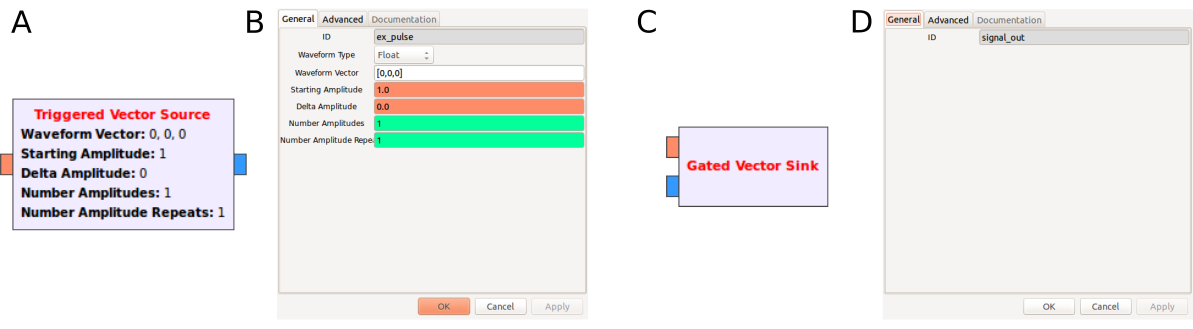
\includegraphics[width = \textwidth,trim=0 0 0 0,clip=false]{triggered_vector_source.png}
\caption{\textcolor{black}{A) \textit{Triggered Vector Source} GNU Radio block.  The orange box on the left represents the block's input node and the blue box on the left represents the output. B) The \textit{Triggered Vector Source} block settings.  C) \textit{Gated Vector Sink} GNU Radio block.  The blue box on the left represents the complex data input node, and the orange box represents the gate controlling the writing of data. D) The \textit{Gated Vector Sink} block settings.}}
\label{fig:tvs}
\end{center}
\end{figure}

GNU Radio was designed for continuous operation, so two custom blocks were developed to enable the sequencing necessary for MRI, which are included in the gr-MRI package.  The first custom block is called the \textit{Triggered Vector Source}, shown in Figure~\ref{fig:tvs}, and plays a specified waveform stored in a python vector whenever its input is high.  During normal MRI scan operation, a square wave with period equal to TR triggers the block to play a predefined pulse.  The settings, shown in Figure~\ref{fig:tvs}(B) allow for control amplitude stepping for the phase encode gradient and RF chopping, and how many times to repeat each step to accommodate averaging.

The second custom block is the \textit{Gated Vector Sink}, shown in Figure~\ref{fig:tvs}(C), which writes a complex data stream on its first input (shown as the blue box) to a python vector whenever its second input (shown as the orange box) is high.

\begin{figure}[ht]
\begin{center}
\includegraphics[width = \textwidth,trim=0 0 0 0,clip=false]{FID_TX_flow.png}
\caption{\textcolor{black}{Pulse transmit section of GNU Radio flowgraph for Pulse and Acquire FID sequence}}
\label{fig:txflow}
\end{center}
\end{figure}

Figure~\ref{fig:txflow}  shows the GNU Radio flow graph for the pulse and acquire FID pulse sequence.  The red box labeled A contains the signal generator that produces a square wave with period equal to the repetition time, or TR.  That signal triggers the Triggered Vector Sources, labeled B, which are each loaded with a waveform and settings that were defined in the gr-MRI script. In this case, the gr-MRI program creates a 100 microsecond hard pulse, and defines a physical readout window that will be fed back into a receive port.  We must create a physical readout window because USB latency makes it impossible to know when the pulses are actually transmitted.  The box labeled C creates the TXE pulse which is sent to unblank the RF Amplifier.  The RF pulse is sent through a moving average filter and is thresholded to create a square pulse that is 10 samples longer than the RF pulse.  The other pulses are delayed by 5 samples to center the RF pulse in the TXE window.  The outputs from the Triggered Vector Sources and TXE pulse are combined into complex signals to be sent out of specific ports of the USRP1s defined in the USRP Sink blocks on the far right, labeled D.  Delays before the USRP Sinks allow for synchronization of the two radios.  Certain settings, such as the device serial addresses, center frequencies, and clock sources are defined within the USRP Sinks.

\begin{figure}[ht]
\begin{center}
\includegraphics[width = \textwidth,trim=0 0 0 0,clip=false]{FID_RX_flow.png}
\caption{\textcolor{black}{RF Receive section of GNU Radio flowgraph for Pulse and Acquire FID sequence}}
\label{fig:rxflow}
\end{center}
\end{figure}

Figure~\ref{fig:rxflow} shows the receive chain for the FID sequence.  The far left block, labeled A, is called the USRP Source and creates a stream of data that was received from the ADC.  The top stream created is the complex RF data received from the preamplifier, and the bottom stream is the complex data recovered from the readout window.  The readout window serves two purposes in receive mode.  First, it defines the acquisition data that is sent back to the gr-MRI script through the gated vector sink (C), and second, it is used to create phase consistency by multiplying the conjugate of the readout window by the raw received data.  The far right block, labeled D, is the QT GUI Sink that is used to show the received signal in real time.  The GUI is shown in Figure~\ref{fig:gui}.

\begin{figure}[!ht]
\begin{center}
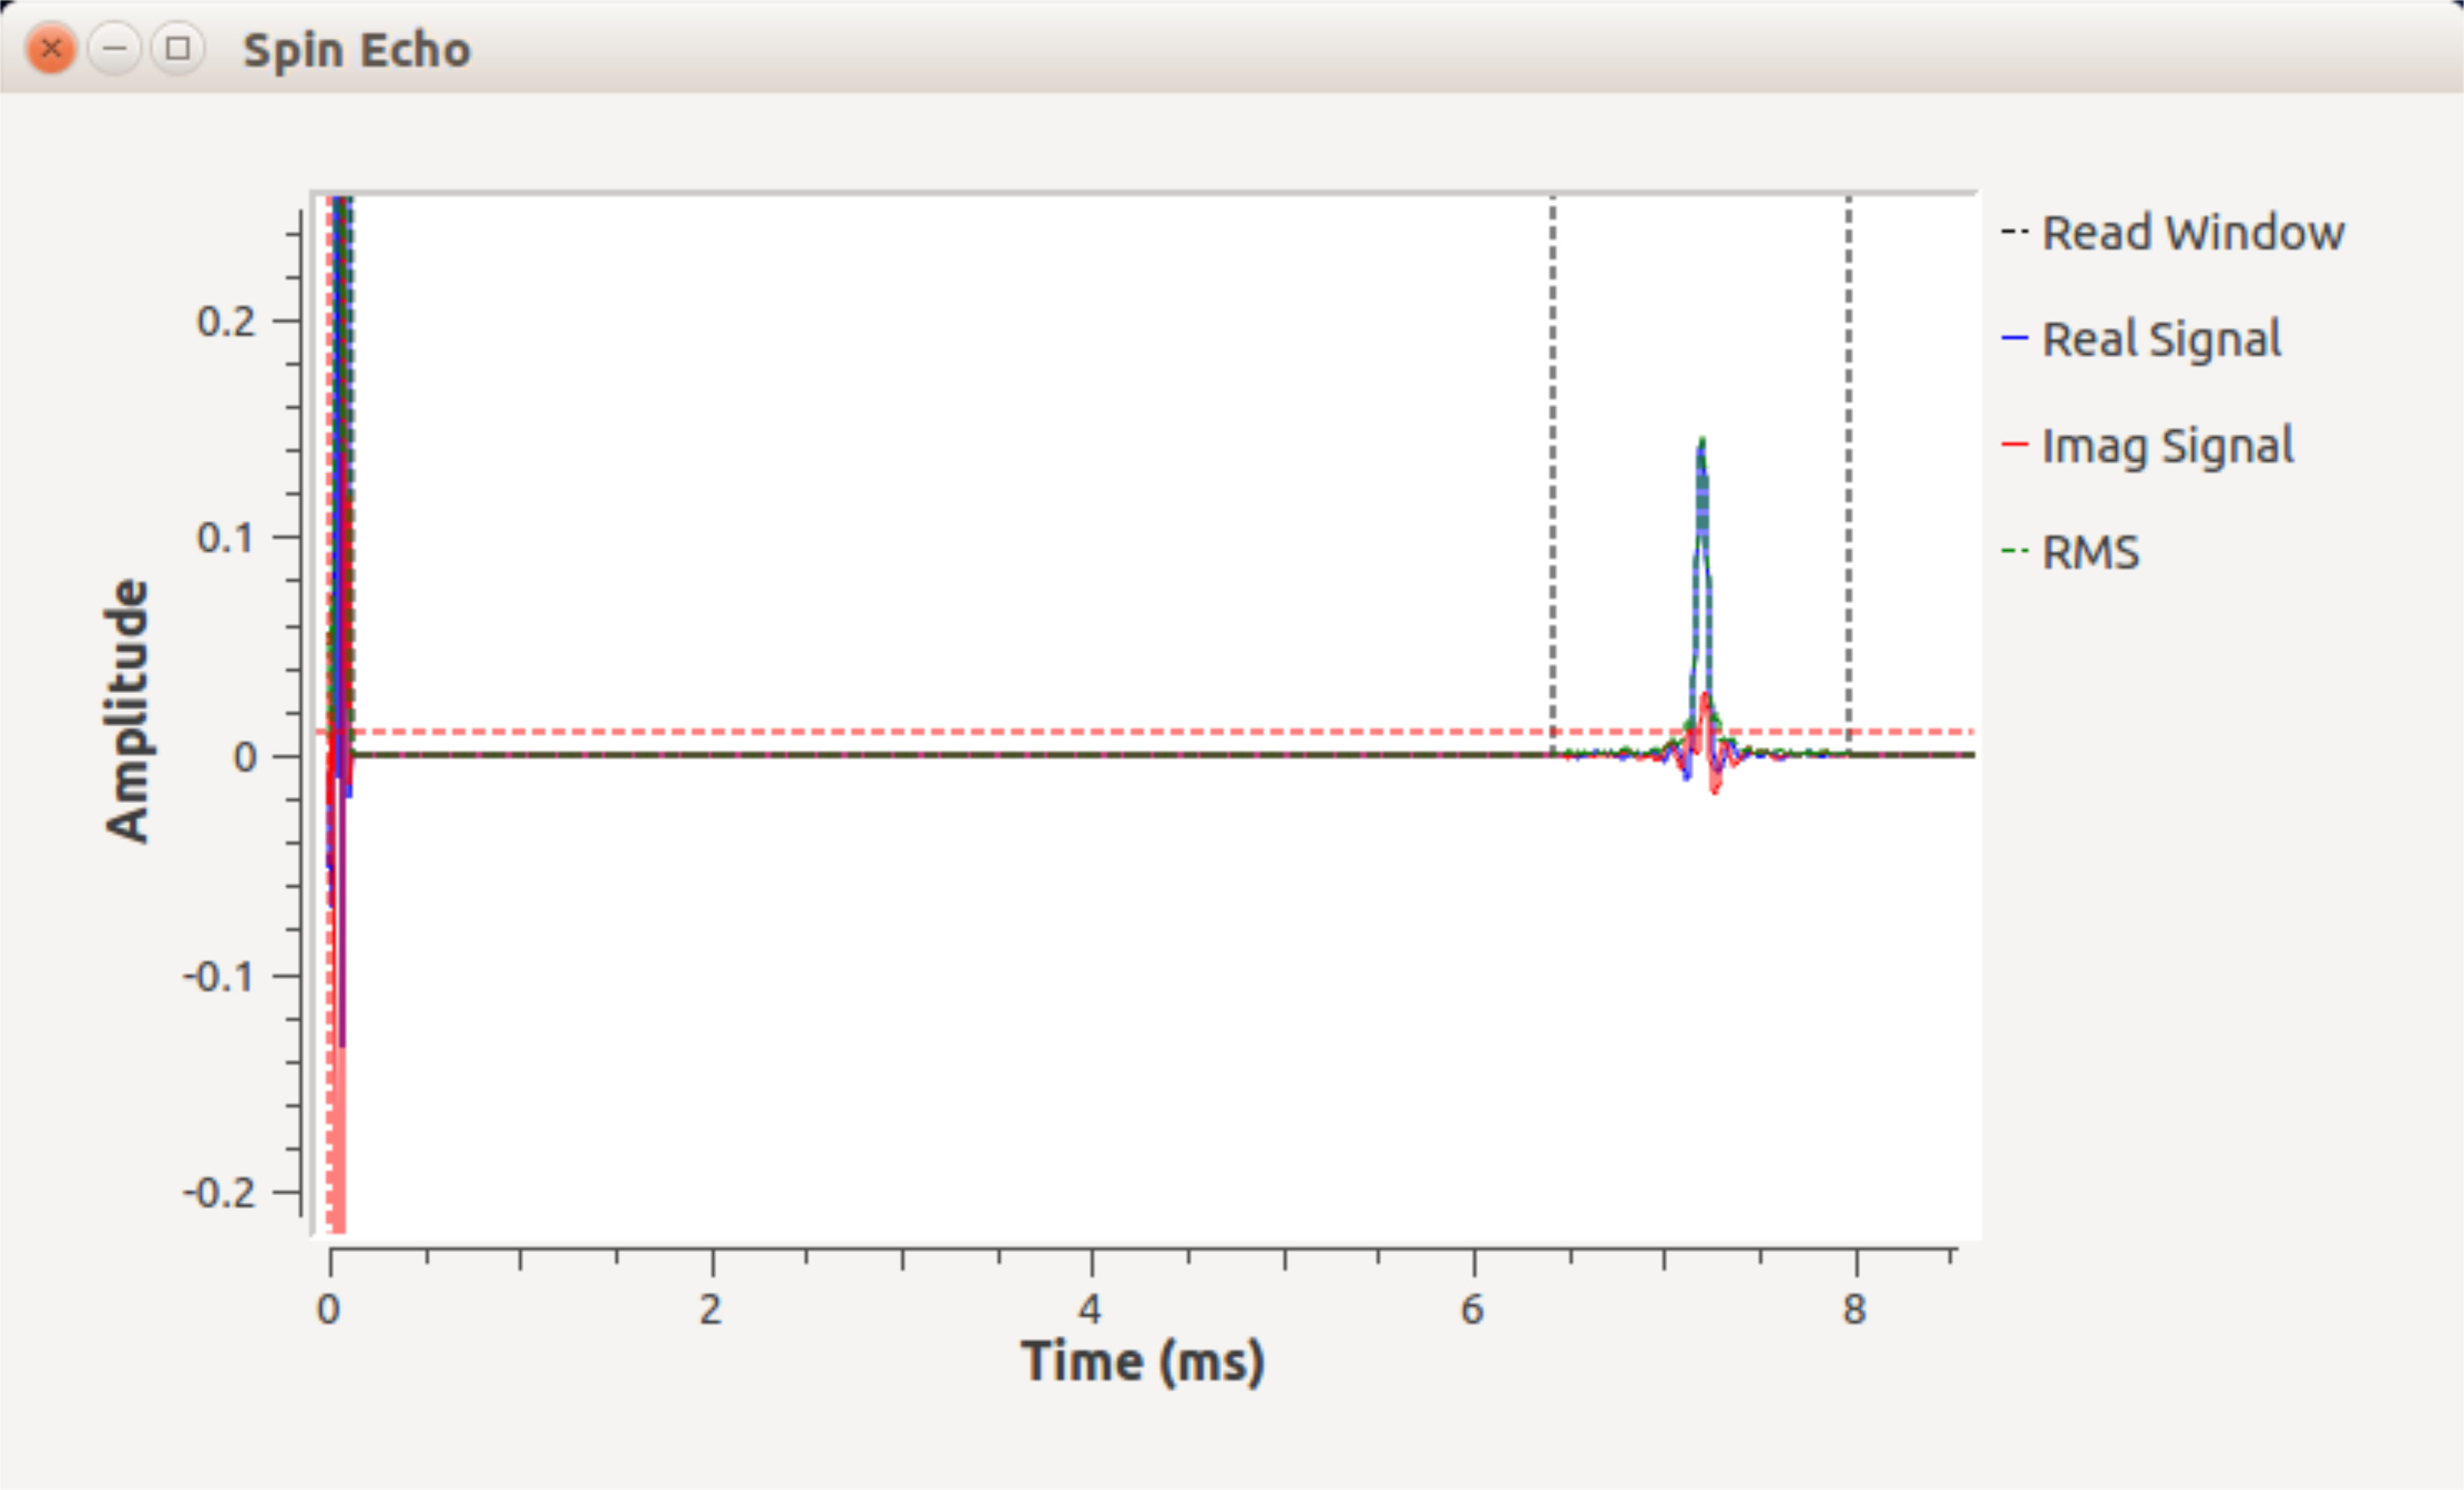
\includegraphics[width = 1\textwidth,trim=0 0 0 0,clip=false]{scan_screenshot.png}
\caption{\textcolor{black}{RX data is shown in real time in the QT GUI window of GNU Radio}}
\label{fig:gui}
\end{center}
\end{figure}

\subsection{Software Organization}\label{Software Organization}

\begin{figure}[ht]
\begin{center}
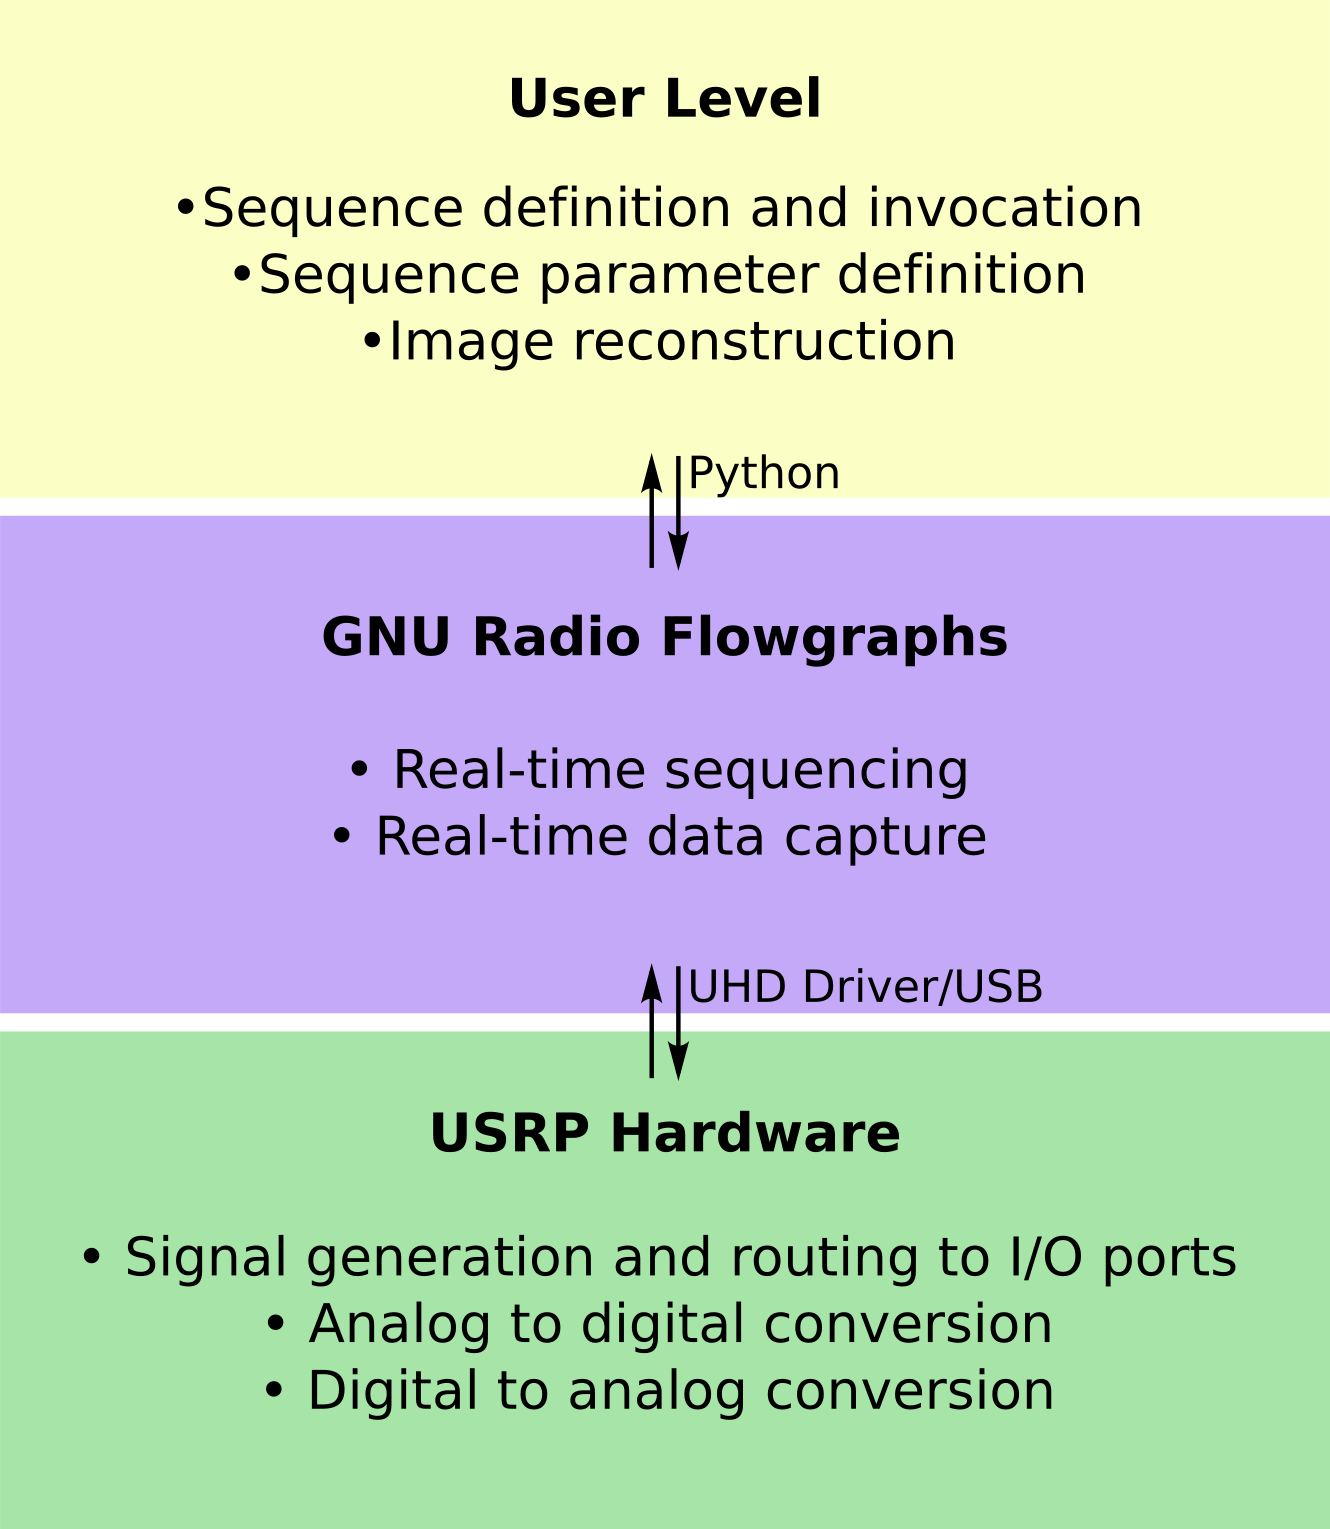
\includegraphics[width = .5\textwidth,trim=0 0 0 0,clip=false]{overview.png}
\caption{\textcolor{black}{Diagram showing the high level organization of the gr-MRI software package}}
\label{fig:overview}
\end{center}
\end{figure}


\indent All pulses necessary to define and control pulse sequences and external hardware are defined in python, and the program pulls sequence parameters from calibration files and config files.  These pulses include RF pulses, gradient amplifier unblanking pulses (TXE), readout window, three DC gradients, and a synchronizing pulse used to synchronize the outputs of the two connected USRP1s.  The gr-MRI software runs a GNU Radio program which times and maps pulses to physical ports on the USRP1.  The GNU Radio program also controls functions such as repeating pulses for averaging, stepping through phase encodes, and defining when to acquire data.  The gr-MRI scripts format and averages raw acquired data as it is acquired.  Simple 2D IFFT reconstruction can be done within the program, or the k-space data can be saved and processed externally.

\subsection{Radio Synchronization}\label{Radio Synchronization}

\begin{figure}[ht]
\begin{center}
\includegraphics[width = \textwidth,trim=0 0 0 0,clip=false]{FID_sync_flow.png}
\caption{\textcolor{black}{Synchronization section of GNU Radio flowgraph}}
\label{fig:syncflow}
\end{center}
\end{figure}

\indent Due to the relatively long delays created by latency, radio synchronization can be an issue.  The USRP1 uses a USB interface that can have latency differences on the order of a few milliseconds, so it is important to synchronize the outputs of the two radios.  To overcome this obstacle, the gr-MRI package uses a port on each radio to send a 10 sample, rectangle synchronization pulse each TR, which is fed back to receive ports on the slaved USRP1.  Figure~\ref{fig:syncflow} shows the synchronizing blocks used in GNU Radio.  The received synchronization pulses are each converted to data streams in the USRP Source, thresholded, and converted to a single complex signal that is stored in a vector sink on the far right.  A function, called  \texttt{sync()} in any calibration or imaging sequence compares the delay between when each pulse is received and sets global master and slave delays to align the transmitted pulses.  This function is automatically run at the beginning of each pulse sequence, and must be called again if the radios become desynchronized.  The blocks at the bottom of the flow graph store error messages to python vectors whenever an desynchronization is detected.  This is used to quickly correct pulse timing if the radios become desynchronized during a scan.


\subsection{Pulse Calibration}\label{Pulse Calibration}

%\begin{figure}[!ht]
%\begin{center}
%\includegraphics[width = .75\textwidth,trim=0 0 0 0,clip=false]{calibimg.png}
%\caption{\textcolor{black}{Calibration caption}}
%\label{fig:foobar}
%\end{center}
%\end{figure}

\indent The gr-MRI software includes two auto-calibration scripts based on a simple pulse and acquire FID pulse sequence.  The first, shown in a, calculates the necessary center frequency offset to add to the system to find the true resonant frequency.  The user specifies the desired number of averages to use for the reading, and the system displays the resultant FFT of the averaged signal, along with a fit Lorentzian curve.  The new center frequency offset is the frequency corresponding to the peak of the Lorentzian curve.  This calibration can be run multiple times to hone in on the true center frequency, but once is typically good enough for imaging.

The second calibration, shown in b, finds the necessary RF pulse amplitude to achieve a 90 degree flip angle.  The user also specifies the desired number of averages, and the script steps through different pulse amplitudes until a maximum received signal amplitude has been reached.  Both scripts save the optimized parameters to a python pickle file named cal.pkl.

\subsection{Gradient Calibration}\label{Gradient Calibration}

\indent The gr-MRI package also has a built in automatic gradient calibration script which uses a spin echo sequence to define gradient strength in each direction.  The user defines the direction to calibrate, and the object size in that dimension. The sequence then calculates the gradient strength based on standard gradients and the resultant bandwidth of the signal.  Gradient strengths are saved in units of G/mm to a python pickle file named gcal.pkl and are used during imaging sequences to convert parameters of FOV and matrix size to gradient pulse output amplitude.

%%%%%%%%%%%%%%%%%%%%%%%%%%%%%%%%------- Hardware -------%%%%%%%%%%%%%%%%%%%%%%%%%%%%%%%%

\section{Hardware Overview}\label{Hardware Overvew}

\indent The gr-MRI software package is compatible with any GNU Radio compatible software-defined radio, and a full list can be found at https://gnuradio.org/redmine/projects/gnuradio/wiki/Hardware.  The work shown in this manuscript used two synchronized Ettus Research USRP1 radios with slaved clocks.  The USRP1 has 4 transmit ports and 4 receive ports per motherboard.  GNU Radio connects to the USRP1 via USB cable to download the pulse sequence to an Altera Cyclone FPGA (0-60Hz) that can create any arbitrary waveform.   A 14 bit (-1V to 1V), 128 Ms/sec digital to analog converter creates the signal, which is passed through software controlled amplifiers, attenuators, and filters.  The received signal also passes through filters, attenuators and amplifiers and is digitized by a 12 bit (-1V to 1V), 64 Ms/sec ADC.  For our case the master radio produces the RF signals and readout window, and the slaved radio produces the DC hardware control pulses and gradient pulses.  The table below shows the pulses created for a typical imaging sequence, as well as the specific port used, and the destination of that signal.  The naming convention for the channel used is \textit{TX/RX Daughterboard\_Slot A or B\_Channel A or B}. Each pulse and its scheduling is defined in the gr-MRI software package and sent to GNU Radio, where the pulse is mapped to a physical port.

\begin{center}
\begin{tabular}[c]{| c | c | c | c |}
	\hline
	\textbf{Pulse} & \textbf{Radio/Channel} & \textbf{Input/Output} & \textbf{Destination} \\ \hline
	RF  & master TX\_A\_A & output & RF Amplifier\\ \hline
	Readout & master TX\_B\_B & output & feedback to master RX\_B\_B\\ \hline
	RF Sync & master TX\_B\_A & output & feedback to slave RX\_A\_A\\ \hline
	RF Receive & master RX\_A\_A & input & n/a\\ \hline
	Gx Gradient & slave TX\_B\_B & output & Gradient Amplifier\\ \hline
	Gy Gradient & slave TX\_A\_A & output & Gradient Amplifier\\ \hline
	Gz Gradient & slave TX\_A\_B & output & Gradient Amplifier\\ \hline
	DC Sync & slave TX\_A\_A & output & feedback to slave RX\_B\_A\\ \hline
	TX Enable & slave TX\_A\_A & output & RF amplifier\\ \hline
\end{tabular}
\end{center}

It is important to note some hardware manipulation that was necessary to enable full hardware control.  The DC synchronization and TXE pulses were compressed into one port by simply adding the waveforms together in GNU Radio.  The output from that port was split and sent in two directions\:  The first direction fed back to the Slave RX\_B\_A (synchronization) port with a 1M$\Omega$ current limiting resistor in line.  The second direction drove a transistor switch that connected the radio 6V voltage supply to the TXE control port on the RF Amplifier.  This was necessary because the maximum voltage output of the SDR is 1V which does not clear the 3.3V necessary to unblank the RF Amplifier used during these experiments.  Other solutions would be to simply amplify the output of that port to reach the necessary voltage requirement, or to use hardware that has a lower turn-on voltage.  Other hardware manipulation may need to be done depending on specific hardware setup, however that is left up to the user.

%%%%%%%%%%%%%%%%%%%%%%%%%%%%%%%%------- Work Flow -------%%%%%%%%%%%%%%%%%%%%%%%%%%%%%%%%

\section{Work Flow}\label{Work Flow}
\begin{figure}[!ht]
\begin{center}
\includegraphics[width = \textwidth,trim=0 0 0 0,clip=false]{workflowfig.png}
\caption{\textcolor{black}{workflow caption}}
\label{fig:workflow}
\end{center}
\end{figure}

\indent Figure~\ref{fig:workflow}  shows the basic workflow of using the gr-MRI package.  The diagram shows a general work step, and the output that the step affects or the input that the step receives.  Program calls are in parentheses below the workflow step.  The figure uses the program slicespin.py as an example for file naming purposes.  Imaging experiments using any gr-MRI sequence or custom built sequence will follow the following steps: (1) Pulses are calibrated parameters are saved using calibrate.py as described in the calibration section above.  This should be done for each new coil, or if the user thinks that either the center frequency or power needed for a 90° flip has changed.  The gradient strengths also need to be calibrated, however this generally only needs to be done once, or if the user thinks that the gradient outputs have changed. (2) The user closes the calibration script and calls the desired imaging sequence program, which in this case is slicespin.py.  The parameters found in the calibration sequence are automatically updated in the pulse sequence. (3) The user can dynamically change sequence parameters or load saved parameters.  The raw signal readout is opened in a new GNU Radio window, and the user can see how the parameter changes affect the signal. (4) The user runs functions to calibrate the final gradients to center the signal in the acquisition space.  (5) The user runs the sequence.  The raw signal from each acquired line of k-space shows up in the GNU Radio window so the user can monitor the scan.  The script also outputs the current line of acquisition, so the user knows how much of the scan has been completed.  (6) The user can choose to save the raw k-space data for external reconstruction, or call a function that performs a simple 2D IFFT image reconstruction.  (7) The user can choose to save data or parameters, change parameters, or begin a new scan.




%%%%%%%%%%%%%%%%%%%%%%%%%%%%%%%%------- RESULTS ------%%%%%%%%%%%%%%%%%%%%%%%%%%%%%%%%
\section{Results}

\begin{figure}[!ht]
\begin{center}
\includegraphics[width = 1\textwidth,trim=0 0 0 0,clip=false]{gre_results.png}
\caption{\textcolor{black}{(A) Slice selective gradient echo pulse sequence created by gradecho.py in gr-MRI software package used to acquire (B) a 4mm thick, 128x128 image. (C) Comparative gradient echo image acquired on Maran system.}}
\label{fig:gre_image}
\end{center}
\end{figure}
 
\indent Figure~\ref{fig:gre_image} shows (A) The pulse sequence created by the stock gradient echo sequence, gradecho.py, and (B) the resulting image with 3 averages.  The excitation pulse was a TBW 8 hamming windowed sinc pulse, played with a gradient in the z direction creating a 4mm slice.  The echo time (TE) was 1.2ms, and the dwell time was 24µs.  The matrix size was 128x128 with a FOV of 20mm in both directions. (C) shows the same sequence, with unknown slice thickness, on the Maran imaging system to confirm that there are no distortions created by the SDR imaging sequence.  There are some chemical shift artifacts in the readout direction, shown as the vertical dimension in the images, in both SDR and Maran images.

\begin{figure}[!ht]
\begin{center}
\includegraphics[width = 1\textwidth,trim=0 0 0 0,clip=false]{se_results.png}
\caption{\textcolor{black}{(A) Slice selective spin echo pulse sequence created by slicespin.py in gr-MRI software package used to acquire (B) a 4mm thick, 128x128 image. (C) Comparative spin echo image acquired on Maran system.}}
\label{fig:se_image}
\end{center}
\end{figure}

\indent Figure~\ref{fig:se_image} shows (A) the pulse sequence created by the stock spin echo sequence, slicespin.py, and (B) the resulting image with 3 averages.  The excitation pulse was also a TBW 8 hamming windowed sinc pulse, with a 4mm slice in the z dimension.  The echo time (TE) was 8ms, and the dwell time was 24µs.  The matrix size was also 128x128 with a FOV of 20mm in both directions. (C) shows the same spin echo sequence, with unknown slice thickness, on the Maran imaging system and we also see no spatial distortion.

\begin{figure}[!ht]
\begin{center}
\includegraphics[width = 1\textwidth,trim=0 0 0 0,clip=false]{ir_results.png}
\caption{\textcolor{black}{(A) Slice selective inversion recover spin echo pulse sequence created by invrecov.py in gr-MRI software package used to acquire (B) a series of 4mm thick, 64x64 images with varying inversion times}}
\label{fig:ir_image}
\end{center}
\end{figure}

\indent Figure~\ref{fig:ir_image} (A) shows the pulse sequence created by the included spin echo inversion recovery sequence, invrecov.py, and (B) the results of varying inverison time (shown as \textit{TI} on the sequence diagram) in a 15 mm sunflower seed oil phantom.  The images have a matrix size of 64x64 over a FOV of 20mm with a 4mm slice in the z dimension.  The signal is nulled at roughly 100ms, which reflects an expected $T_1$ of approximately 150 ms.

%%%%%%%%%%%%%%%%%%%%%%%%%%%%%%%%-------- DISCUSSION --------%%%%%%%%%%%%%%%%%%%%%%%%%%%%%%%%
\section{Discussion}
\indent


%%%%%%%%%%%%%%%%%%%%%%%%%%%%%%%%------- CONCLUSION -------%%%%%%%%%%%%%%%%%%%%%%%%%%%%%%%%
\section{Conclusion}
\indent The gr-MRI package and SDR hardware aims to alleviate some of the major issues present in existing MRI spectrometers, which are often expensive, inflexible, and run non-intuitive software.  The package lowers barriers to home-building MRI consoles and quickly implementing stock, or custom pulse sequences.  It has shown the ability to produce high fidelity signals, which enable the acquisition of high resolution images using the three pre-built pulse sequences, and has the capacity to create more complex sequences and pulse shapes.

The full package and set up instructions are free for use and can be downloaded at...

\section*{Acknowledgments}

This work was supported by NIH R21 EB 018521.

%%%%%%%%%%%%%%%%%%%%%%% REFERENCES %%%%%%%%%%%%%%%%%%%%%%%%%%%%


%%%%%%%%%%%%%%%%%%%%%%%%%%%%%%%%------- REFERENCES -------%%%%%%%%%%%%%%%%%%%%%%%%%%%%%%%%

\section*{References}
\bibliography{gnuradio_mri}{}
\bibliographystyle{plain}

\end{document}

 
 
 
 
